\section{Analysis of PREFLEX balancing algorithm}
\begin{comment}

In this section we are going to evaluate the performance of the algorithm for different configuration parameters. 

\subsection{Algorithm modes}

PREFLEX balancing algorithm could be configured according to the approach that we want to implement. This is done by setting a coefficient for each mode. $\beta_{E}$, $\beta_{C}$ and $\beta_{L}$ denotes the positive factors associated consecutively with Equalization $E$,  Conservative $C$, and Loss Driven$L$ modes.


\begin{figure}[h]
\begin{center}

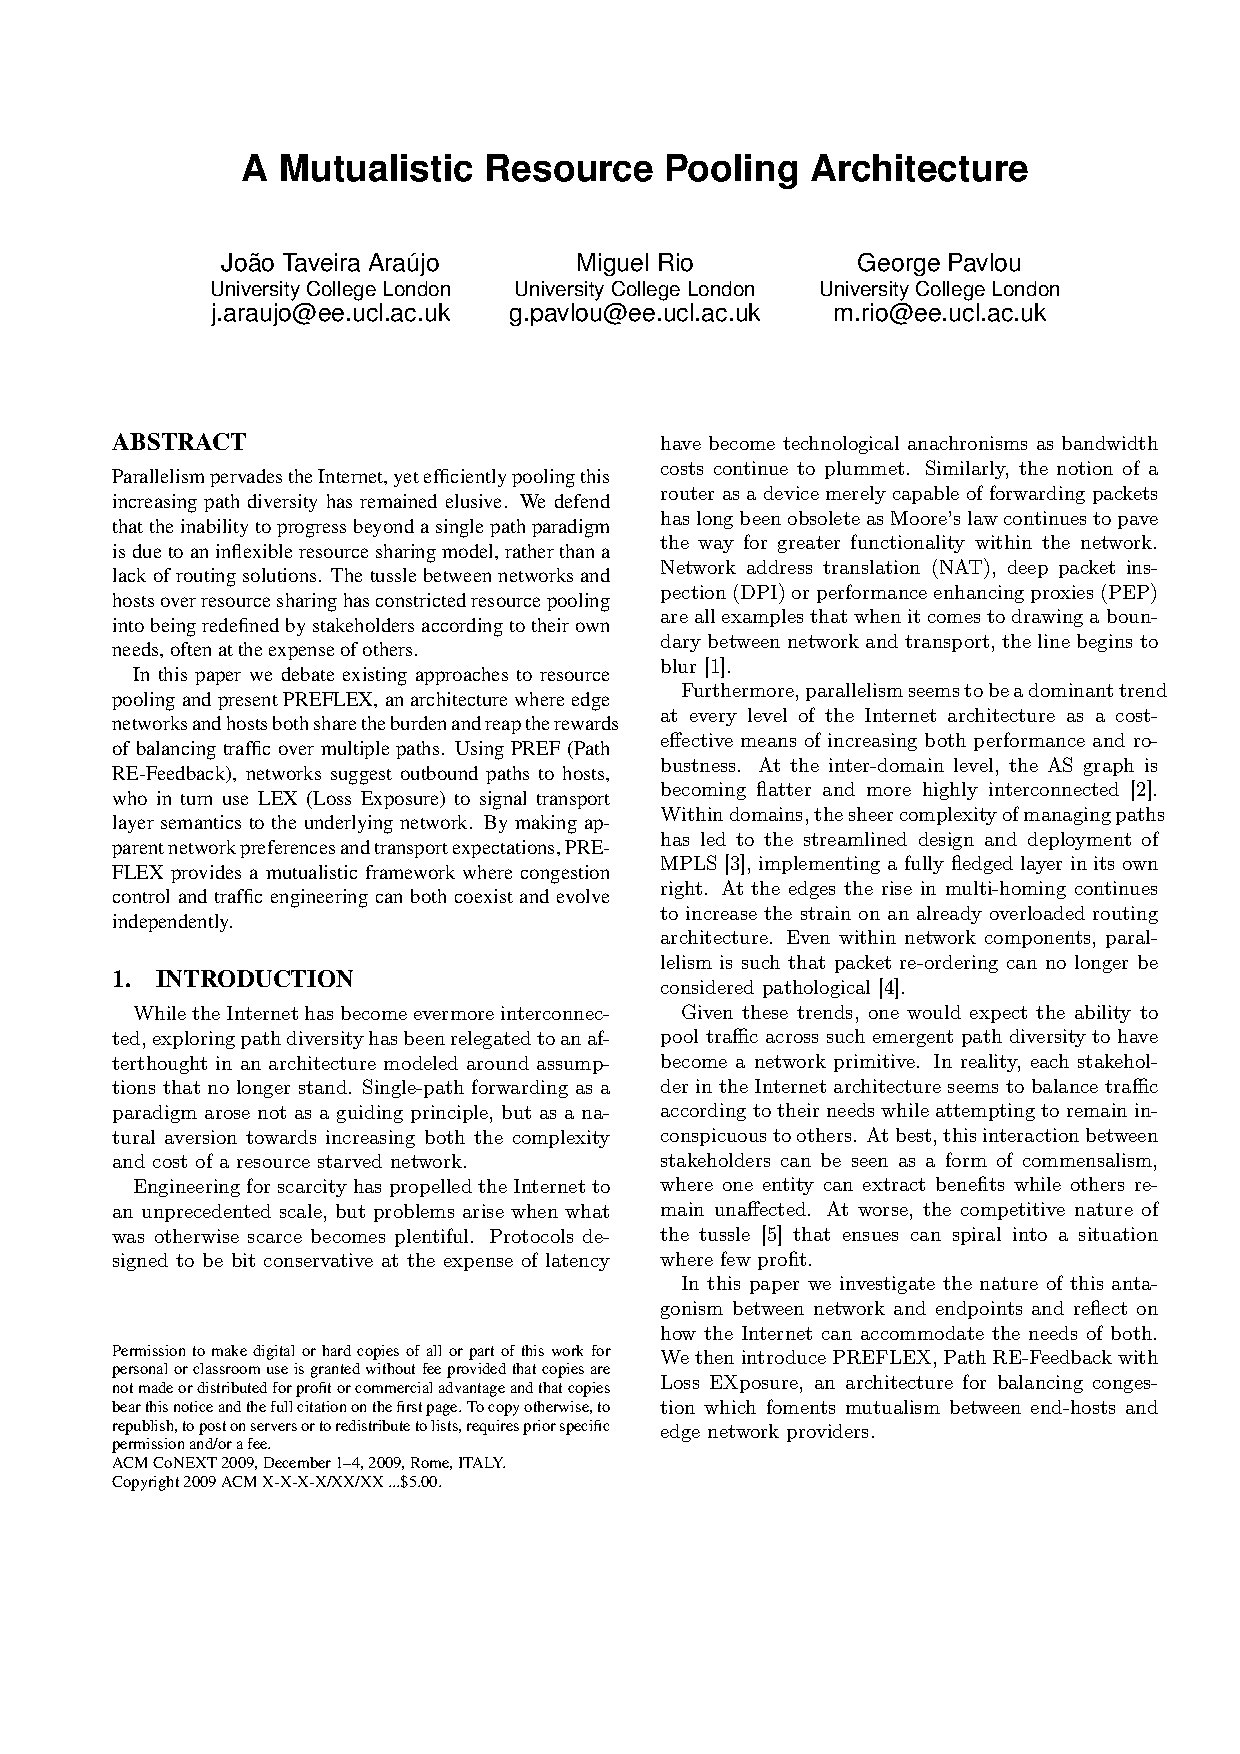
\epsfig{file=img/eps/rearch, width=4.5in}
\caption{

Network Topology.
   \label{fig:topo332}
}
\end{center}
\end{figure}

\subparagraph{Simulation scenario} Figure \ref{fig:topo332} shows the topology used for the simulations, and figure \ref{fig:flowA} shows how traffic evolve. During the scenario a failure happens between 600sec and 650 sec and E2 can't be reach through Link 1.

\begin{figure}[h!]
\begin{center}

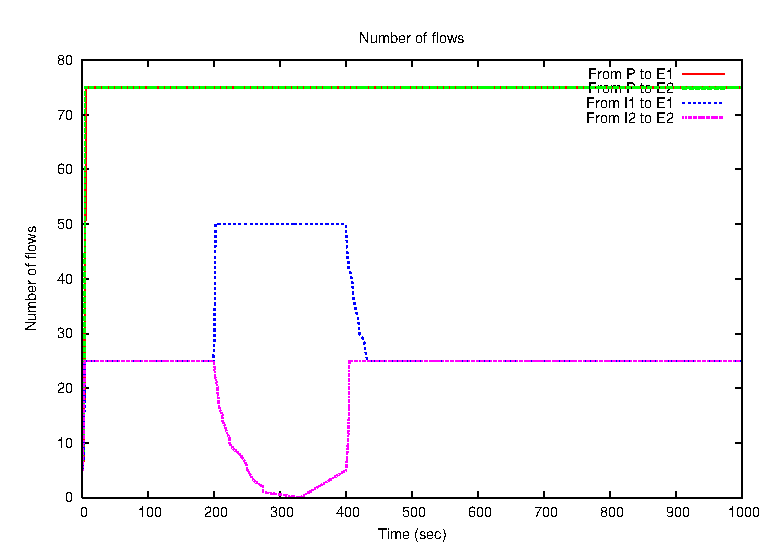
\epsfig{file=img/flowAlt, width=4.5in}
\caption{

Flow Numbers.

   \label{fig:flowA}
}
\end{center}
\end{figure}

\clearpage

{\bf Conservative mode} : $\beta_{E}=0$, $\beta_{C}=1$ and $\beta_{L}=0$
\\The conservative mode doesn't achieve an accurate congestion balancing over the available paths (figure \ref{fig:splitCon-loss}). But more importantly, the split as desired by the balancer in this mode is not stable(figure \ref{fig:splitCon-fwnd}). Thus, it can't be used to stabilize the performance of the balancer. A plausible explanation is the  limitation of the assumption that the flow fraction is equal to byte fraction, when the loss rates of paths aren't equivalent.

\begin{figure}[h!]
\begin{center}

\epsfig{file=img/sec-5-2-2/Alt-split-0-100-0/loss-192-0-0-0, width=4.5in}
\caption{
  Loss ratio $\rho_{i}$ for destination E1 as seen by balancer P in consrvative mode.

   \label{fig:splitCon-loss}
}
\end{center}
\end{figure}

\clearpage
\begin{figure}[h!]
\begin{center}

\epsfig{file=img/sec-5-2-2/Alt-split-0-100-0/fwnd-192-0-0-0, width=4.5in}
\caption{
  The desired split that balancer P set for destination E1 in conservative mode.

   \label{fig:splitCon-fwnd}
}
\end{center}
\end{figure}


{\bf Equalization} : $\beta_{E}=1$, $\beta_{C}=0$ and $\beta_{L}=0$
\\As depicted by figure \ref{fig:splitEqual-loss}, an equal distribution of flows over the paths doesn't achieve an equal balancing of loss. Moreover, its performance depends on the traffic nature in the network. Path 3 is underutilized and  illustrates the suboptimal nature of equal balancing. Also the difference of congestion levels in the other two paths is directly linked to changes in traffic demand. During the change on traffic demand between time 200sec and 600sec, the difference between the congestion levels significantly increased.

However, the real contribution of the "equal" mode in PREFLEX balancing is to ensure that a minimum number of flows are sent over each path. In fact, as we are going to see next, the accuracy of the loss estimation made by the balancer depends on the number of flows sent over the path. 

\clearpage
\begin{figure}[h]
\begin{center}

\epsfig{file=img/sec-5-2-2/Alt-split-0-0-100/loss-192-0-0-0, width=4.5in}
\caption{
  Loss ratio $\rho_{i}$ for destination E1 as seen by balancer P in equalisation mode.

   \label{fig:splitEqual-loss}
}
\end{center}
\end{figure}


{\bf Unbounded loss driven mode} : $\beta_{E}=0$, $\beta_{C}=0$ and $\beta_{L}=1$
\\Figures \ref{fig:splitpureLoss-fwnd1} and \ref{fig:splitpureLoss-fwnd1} show that the balancer allocates different splits for destination E1 and E2 even when the system is symmetric for the two destinations. This is explained by the fact that balancing for the two destinations is processed separately. It is logical since the paths for the two destinations are different even if they share the same bottleneck in our topology. We should also keep in mind that that there are more than one optimal split. In the simulation topology,  the three links have the same capacity and thus during the first 200sec the two destinations have the same number of flows. Though we might expect that it'll allocate the split in the same way for both destinations. This is not problematic since the balancer manages though to well balance the loss during the first 200sec (see \ref{fig:splitpureLoss-loss1} and \ref{fig:splitpureLoss-loss2}). 
But by keeping to send less E2 flows on path 3, the accuracy of the loss estimation  becomes low and different from E1 flows. In particular, it is over estimated what accelerate more the drop (the peaks of path 3 loss in figure \ref{fig:splitpureLoss-loss2}). As a result the equalization mode is used to make sure that there are enough flows on every path for an accurate estimation of the loss.

\begin{figure}[h]
\begin{center}

\epsfig{file=img/sec-5-2-2/Alt-split-100-0-0/fwnd-192-0-0-0, width=4.5in}
\caption{
  The desired split that balancer P set for destination E1 in unbounded loss driven mode.

   \label{fig:splitpureLoss-fwnd1}
}
\end{center}
\end{figure}

\begin{figure}[h]
\begin{center}

\epsfig{file=img/sec-5-2-2/Alt-split-100-0-0/fwnd-192-0-1-0, width=4.5in}
\caption{
  The desired split that balancer P set for destination E2 in unbounded loss driven mode.

   \label{fig:splitpureLoss-fwnd2}
}
\end{center}
\end{figure}


\begin{figure}[h]
\begin{center}

\epsfig{file=img/sec-5-2-2/Alt-split-100-0-0/loss-192-0-0-0, width=4.5in}
\caption{
  Loss ratio $\rho_{i}$ for destination E1 as seen by balancer P in unbounded loss driven mode.

   \label{fig:splitpureLoss-loss1}
}
\end{center}
\end{figure}

\begin{figure}[h]
\begin{center}

\epsfig{file=img/sec-5-2-2/Alt-split-100-0-0/loss-192-0-1-0, width=4.5in}
\caption{
  Loss ratio $\rho_{i}$ for destination E2 as seen by balancer P in unbounded loss driven mode.

   \label{fig:splitpureLoss-loss2}
}
\end{center}
\end{figure}

\clearpage

{\bf Bounded loss driven mode} : $\beta_{E}=0.9$, $\beta_{C}=0$ and $\beta_{L}=0.1$
\\By allocating a share of the traffic to be equally distributed we guarantee that a minimum number of flows is sent over each path to continue probing the path in question and accurately estimate its level of congestion. The effect of this boundary is clearly shown in the loss distribution compared to the previous mode \ref{fig:splitlossD-loss1} and \ref{fig:splitlossD-loss2}. Though, the  booked share for equalization should be too high to block the loss equalization process. 

The algorithm has also a good answer towards failures. \ref{fig:splitlossD-fwnd1} and \ref{fig:splitlossD-fwnd1} {\bf Something about failure}


\begin{figure}[h]
\begin{center}

\epsfig{file=img/sec-5-2-2/Alt-split-90-0-10/fwnd-192-0-0-0, width=4.5in}
\caption{
  The desired split that balancer P set for destination E1 in bounded loss driven mode.

   \label{fig:splitlossD-fwnd1}
}
\end{center}
\end{figure}

\begin{figure}[h]
\begin{center}

\epsfig{file=img/sec-5-2-2/Alt-split-90-0-10/fwnd-192-0-1-0, width=4.5in}
\caption{
  The desired split that balancer P set for destination E2 in bounded loss driven mode.

   \label{fig:splitlossD-fwnd2}
}
\end{center}
\end{figure}


\begin{figure}[h]
\begin{center}

\epsfig{file=img/sec-5-2-2/Alt-split-90-0-10/loss-192-0-0-0, width=4.5in}
\caption{
  Loss ratio $\rho_{i}$ for destination E1 as seen by balancer P in bounded loss driven mode.

   \label{fig:splitlossD-loss1}
}
\end{center}
\end{figure}

\begin{figure}[h]
\begin{center}

\epsfig{file=img/sec-5-2-2/Alt-split-90-0-10/loss-192-0-1-0, width=4.5in}
\caption{
  Loss ratio $\rho_{i}$ for destination E2 as seen by balancer P in bounded loss driven mode.

   \label{fig:splitlossD-loss2}
}
\end{center}
\end{figure}

\clearpage
\subsection{Decision time interval}

The decision time interval is an external parameter for the algorithm. It determines how often the network domain updates the split. The stability of the algorithm and how long it takes to reach equilibrium is linked to the decision interval. On another hand, this decision interval is also dependant of the period over which the loss signals are aggregated. Consequently, a frequent update of the split may result in an instability of the system that will be even stressed when the aggregation time of the losses is carried out for small periods of time. In practice, we choose the decision time interval to the double of the time value for the aggregation.

The graphs bellow show the dropping rate observed at the bottleneck. 

\begin{figure}[h]
\begin{center}

\epsfig{file=img/sec-5-2-1/eight/dropRate, width=5in}
\caption{
 Drop Rate at the bottlenecks for an update  of  8 sec.
   \label{fig:split-eight}
}
\end{center}
\end{figure}

%FLARE
\begin{figure}[h!]
\begin{center}
\epsfig{file=img/sec-5-2-1/four/dropRate, width=5in}
\caption{
 Drop Rate at the bottlenecks for an update of 4 sec.
   \label{fig:split-time-four}
}
\end{center}
\end{figure}

\clearpage

{\bf Update interval: 1sec}

\begin{figure}[h]
\begin{center}

\epsfig{file=img/sec-5-2-1/one/dropRate, width=5in}
\caption{
 Drop Rate at the bottlenecks for an update  of 1sec.
   \label{fig:split-one}
}
\end{center}
\end{figure}

As expected, with a small update interval the algorithm acts more aggressively and doesn't leave enough time for the flows to reach stability. Consequently,  the congestion level experienced in the different paths (expressed by the dropping rate at each bottleneck) is not well balanced. Larger time intervals (8 and 4 sec) allow loss balancer to achieve a better balancing of the congestion over the available paths and with an enhanced stability. From the different simulations that we've conducted, an update interval between 40 to 100 RTT (approximately 100ms for the simulations here) allowed to achieve most of the time a good accuracy of the congestion balancing. This is only a simulation observation. An even higher value for the update interval turns the balancer too slow. This effect could be illustrated with the reaction of the system for sudden and important changes in traffic demand. We could see at around the second 600, when the demand on traffic turned from a destination to another one, the balancer with an update interval of 4 sec required slightly less time to achieve equilibrium.    

\clearpage

%\begin{figure}[htbp]
%\begin{center}
%\subfloat[]{
%\label{rcpstart4}
%\includegraphics[scale=0.4]{plots/lan/1.5Mb/rcp/flowstart4.eps}}
%\hspace{10mm}
%\subfloat[]{
%\label{xcprcpstart4}
%\includegraphics[scale=0.4]{plots/lan/1.5Mb/xcp0/flowstart4.eps}}
%\caption{The throughput of end-hosts and the router queue as a fourth flow starts, using \protect\subref{rcpstart4} RCP and \protect\subref{xcprcpstart4} XCP.}
%\label{rcpstart4comp}
%\end{center}
%\end{figure}


\end{comment}
